% \section{Overview}

% I/O management is a major component of operating system
% design and operation.

% \begin{itemize}
%   \item Important aspect of computer operation
%   \item I/O devices vary greatly
%   \item Various methods to control them
%   \item Performance management
%   \item New types of devices frequent
% \end{itemize}

% Ports, busses, device controllers connect to various devices.
% Device drivers encapsulate device details, present uniform device-access interface to I/O subsystem

% \section{I/O Hardware}

% Incredible variety of I/O devices such as: storage, trasmission, human interface.

% Common concepts - signals from I/O devices interface with computer:




% \begin{flushleft}
%   \begin{minipage}{0.65\linewidth}
%     \raggedright
%     \begin{itemize}
%       \item \textbf{Port:} - connection point for device
%       \item \textbf{Bus:} - daisy chain or shared direct access
%             \begin{itemize}
%               \item[-] \textbf{PCI:} - bus common in PCs and servers, PCI Express (PCIe)
%               \item[-] \textbf{expansion bus} - connects relatively slow devices
%               \item[-] \textbf{Serial-attached SCSI (SAS)} - common disk interface
%             \end{itemize}
%       \item \textbf{Controller (host adapter)} - electronics that operate port, bus, device:
%             \begin{itemize}
%               \item[-] Sometimes integrated
%               \item[-] Sometimes separate circuit board (host adapter)
%               \item[-] Contains processor, microcode, private memory, bus controller, etc.
%                     Some talk to per-device controller with bus controller, microcode, memory,
%                     etc
%             \end{itemize}
%     \end{itemize}
%   \end{minipage}%
%   \hfill
%   \begin{minipage}{0.3\linewidth}
%     \centering
%     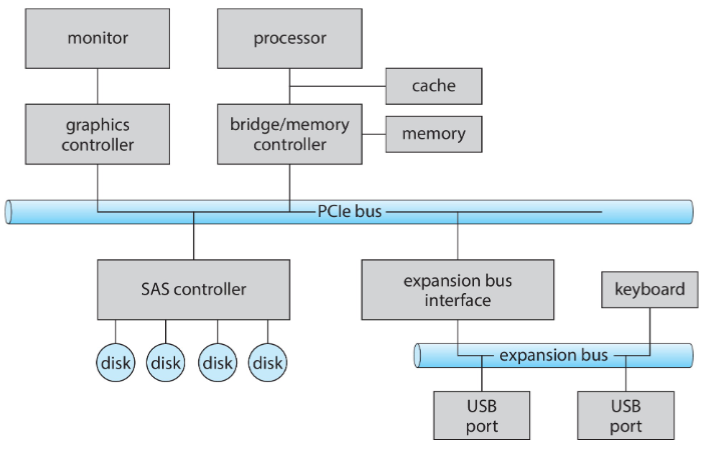
\includegraphics[width=\linewidth]{content/OS_Internals/images/2026-03-31-16-53-40.png}
%   \end{minipage}
% \end{flushleft}


% \begin{flushleft}
%   \begin{minipage}{0.65\linewidth}
%     \raggedright

%     Fibre channel (FC) is complex controller, usually separate
%     circuit board (host-bus adapter, HBA) plugging into bus.

%     I/O instructions control devices.

%     Devices usually have registers where device driver places
%     commands, addresses, and data to write, or read data from
%     registers after command execution

%     \begin{itemize}
%       \item Data-in register, data-out register, status register, control  register
%       \item Typically 1-4 bytes, or FIFO buffer
%     \end{itemize}

%     Devices have addresses, used by: Direct I/O instructions or Memory-mapped I/O (MMIO), device data and command registers mapped to
%     processor address space especially for large address spaces (graphics).


%   \end{minipage}%
%   \hfill
%   \begin{minipage}{0.3\linewidth}
%     \centering
%     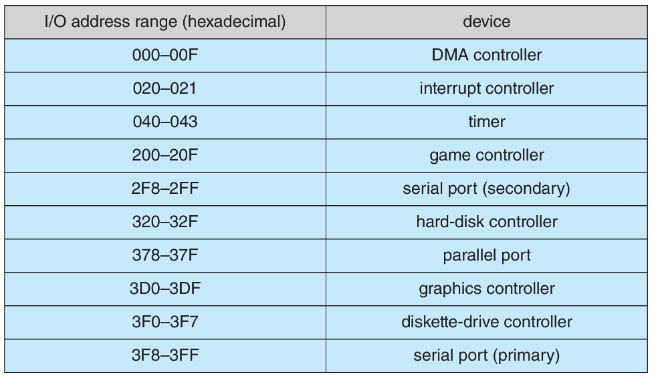
\includegraphics[width=\linewidth]{content/OS_Internals/images/2026-03-31-16-57-08.png}
%     \captionof{figure}{Device I/O Port Locations on PCs (partial)}
%   \end{minipage}
% \end{flushleft}

% \section{Polling}

% For each byte of I/O:

% \begin{enumerate}
%   \item Read busy bit from status register until 0
%   \item Host sets read or write bit and if write copies data into data-out register
%   \item Host sets command-ready bit
%   \item Controller sets busy bit, executes transfer
%   \item Controller clears busy bit, error bit, command-ready bit when transfer done
% \end{enumerate}

% Step 1 is busy-wait cycle to wait for I/O from device. This is reasonable if device is fast but inefficient if device slow.

% CPU switches to other tasks? But if miss a cycle data overwritten / lost

% \section{Interrupts}
% Polling can happen in 3 instruction cycles.
% Read status, logical-and to extract status bit, branch if not zero. How to be
% more efficient if non-zero infrequently?


% CPU Interrupt-request line triggered by I/O device, checked by processor after each instruction

% \begin{itemize}
%   \item \textbf{Interrupt handler} receives interrupts could be \textbf{maskable} to ignore or delay some interrupts
%   \item \textbf{Interrupt vector} to dispatch interrupt to correct handler. Context switch at start and end is based on priority, some non-maskable.
%         Interrupt chaining if more than one device at same interrupt number
% \end{itemize}


% \begin{flushleft}
%   \begin{minipage}{0.65\linewidth}
%     \raggedright

%     Interrupt mechanism also used for exception: terminate process, crash system due to hardware error


%     Page fault executes when memory access error.
%     System call executes via trap to trigger kernel to execute
%     request.

%     Multi-CPU systems can process interrupts concurrently, If operating system designed to handle it.

%     Used for time-sensitive processing, frequent, must be fast


%   \end{minipage}%
%   \hfill
%   \begin{minipage}{0.3\linewidth}
%     \centering
%     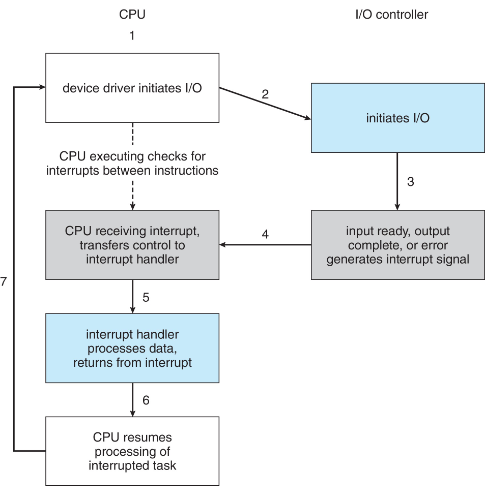
\includegraphics[width=\linewidth]{content/OS_Internals/images/2026-03-31-17-03-06.png}
%   \end{minipage}
% \end{flushleft}


% \section{Latency}

% Stressing interrupt management because even single-user systems
% manage hundreds or interrupts per second and servers hundreds of
% thousands.

% For example, a quiet macOS desktop generated 23,000 interrupts over 10 seconds.

% \section{Direct Memory Access}

% Used to avoid programmed I/O (one byte at a time) for large data
% movement. Requires DMA controller.

% Bypasses CPU to transfer data directly between I/O device and
% memory.


% OS writes DMA command block into memory:

% \begin{itemize}
%   \item Source and destination addresses
%   \item Read or write mode
%   \item Count of bytes
%   \item Writes location of command block to DMA controller
%   \item Bus mastering of DMA controller - grabs bus from CPU. Cycle stealing from CPU but still much more efficient
%   \item When done, interrupts to signal completion
% \end{itemize}

% Version that is aware of virtual addresses can be even more efficient -
% DVMA.

% \section{Six Step Process to Perform DMA Transfer}

% \begin{figure}[h!]
%   \centering
%   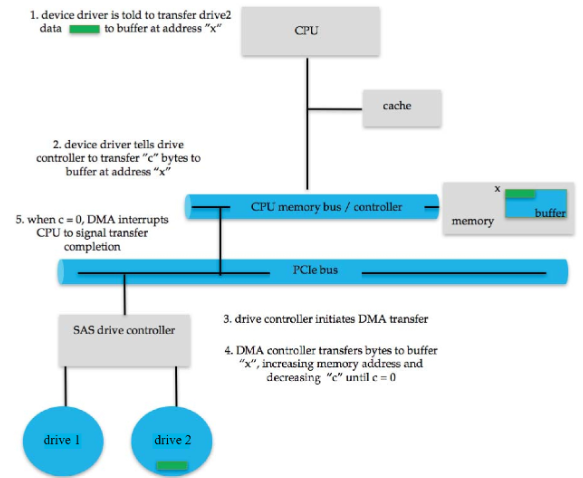
\includegraphics[width=0.5\linewidth]{content/OS_Internals/images/2026-03-31-17-09-14.png}
% \end{figure}


% \section{Application I/O Interface}

% I/O system calls encapsulate device behaviors in generic classes.
% Device-driver layer hides differences among I/O controllers from kernel.
% New devices talking already-implemented protocols need no extra work.
% Each OS has its own I/O subsystem structures and device driver frameworks.
% Devices vary in many dimensions:

% \begin{itemize}
%   \item Character-stream or block
%   \item Sequential or random-access
%   \item Synchronous or asynchronous (or both)
%   \item Sharable or dedicated
%   \item Speed of operation
%   \item read-write, read only, or write only
% \end{itemize}

% \begin{figure}[h!]
%   \centering
%   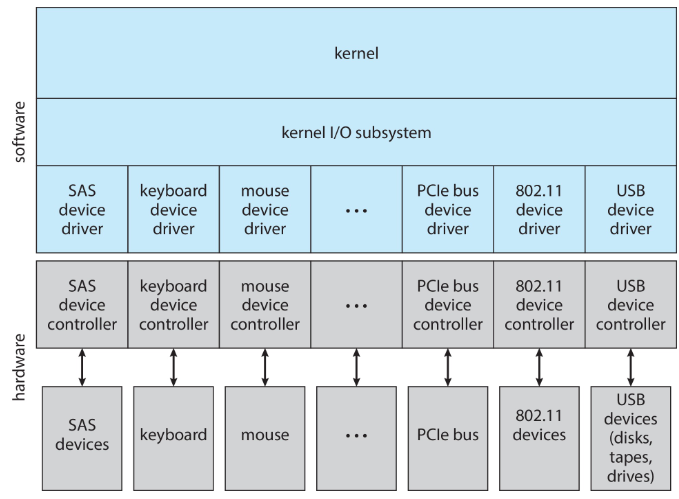
\includegraphics[width=0.5\linewidth]{content/OS_Internals/images/2026-03-31-17-11-50.png}
% \end{figure}

% \section{Characteristics of I/O Devices}

% \begin{table}[h!]
%   \renewcommand{\arraystretch}{1.5}
%   \centering
%   \begin{tabular}{p{3.5cm} p{5.5cm} p{4.5cm}}
%     \hline
%     \textbf{Aspect}    & \textbf{Variation}                                                                  & \textbf{Example}                                  \\
%     \hline
%     data-transfer mode & character \newline block                                                            & terminal \newline disk                            \\
%     access method      & sequential \newline random                                                          & modem \newline CD-ROM                             \\
%     transfer schedule  & synchronous \newline asynchronous                                                   & tape \newline keyboard                            \\
%     sharing            & dedicated \newline sharable                                                         & tape \newline keyboard                            \\
%     device speed       & latency \newline seek time \newline transfer rate \newline delay between operations &                                                   \\
%     I/O direction      & read only \newline write only \newline read--write                                  & CD-ROM \newline graphics controller \newline disk \\
%     \hline
%   \end{tabular}
% \end{table}


% \begin{figure}[h!]
%   \centering
%   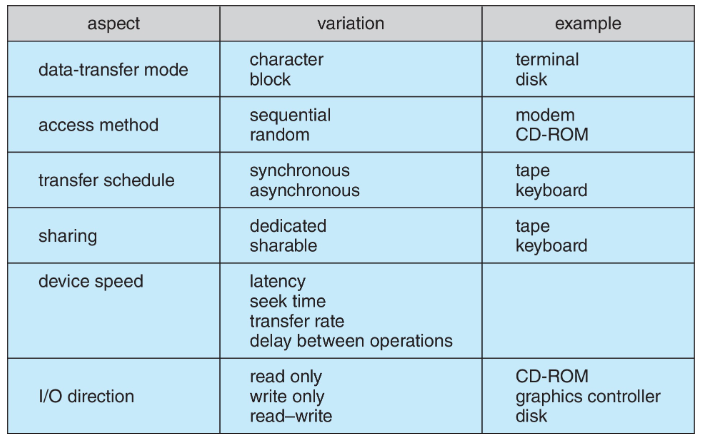
\includegraphics[width=0.5\linewidth]{content/OS_Internals/images/2026-03-31-17-12-50.png}
% \end{figure}


% Subtleties of devices handled by device drivers
% Broadly I/O devices can be grouped by the OS into

% \begin{itemize}
%   \item Block I/O
%   \item Character I/O (Stream)
%   \item Memory-mapped file access
%   \item Network sockets
% \end{itemize}

% For direct manipulation of I/O device specific characteristics, usually an escape / back door
% Unix ioctl() call to send arbitrary bits to a device control register and data to device data register
% UNIX and Linux use tuple of "major" and "minor" device numbers to identify type and instance of devices (here major 8 and minors 0-4):

% \begin{verbatim}
% % ls -l /dev/sda* 
% brw-rw---- 1 root disk 8, 0 Mar 16 09:18 /dev/sda 
% brw-rw---- 1 root disk 8, 1 Mar 16 09:18 /dev/sda1 
% brw-rw---- 1 root disk 8, 2 Mar 16 09:18 /dev/sda2 
% brw-rw---- 1 root disk 8, 3 Mar 16 09:18 /dev/sda3 
% \end{verbatim}

% \section{Block and Character Devices}

% Block devices include disk drives
% \begin{itemize}
%   \item Commands include read, write, seek
%   \item Raw I/O, direct I/O, or file-system access
%   \item Memory-mapped file access possible
%         \begin{itemize}
%           \item[-] File mapped to virtual memory and clusters brought via demand paging
%         \end{itemize}
%   \item DMA
% \end{itemize}

% Character devices include keyboards, mice, serial ports
% \begin{itemize}
%   \item Commands include get(), put()
%   \item Libraries layered on top allow line editing
% \end{itemize}

% \section{Network Devices}

% Varying enough from block and character to have own interface
% Linux, Unix, Windows and many others include socket interface

% \begin{itemize}
%   \item Separates network protocol from network operation
%   \item Includes select() functionality
% \end{itemize}
% Approaches vary widely (pipes, FIFOs, streams, queues, mailboxes)

% \section{Clocks and Timers}

% Provide current time, elapsed time, timer.
% Normal resolution about 1/60 second. Some systems provide higher-resolution
% timers. Programmable interval timer used for timings, periodic interrupts

% \verb|ioctl()| (on UNIX) covers odd aspects of I/O such as clocks and timers

% \section{Nonblocking and Asynchronous I/O}

% \subsubsection{Blocking - process suspended until I/O completed}
% \begin{itemize}
%   \item Easy to use and understand
%   \item Insufficient for some needs
% \end{itemize}

% \subsubsection{Nonblocking - I/O call returns as much as available}
% \begin{itemize}
%   \item User interface, data copy (buffered I/O)
%   \item Implemented via multi-threading
%   \item Returns quickly with count of bytes read or written
%   \item select() to find if data ready then read() or write() to transfer
% \end{itemize}

% \subsubsection{Asynchronous - process runs while I/O executes}
% \begin{itemize}
%   \item Difficult to use
%   \item I/O subsystem signals process when I/O completed
% \end{itemize}

% \section{Two I/O Methods}

% \begin{figure}[h!]
%   \centering
%   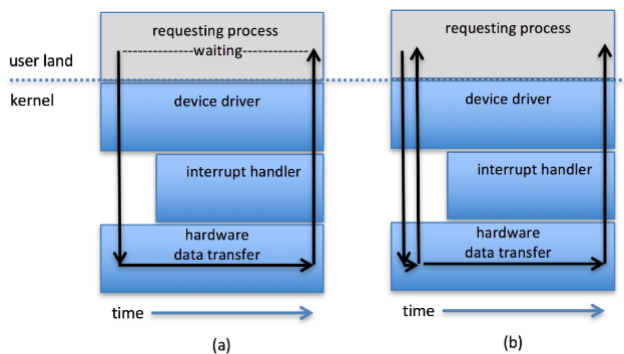
\includegraphics[width=0.4\linewidth]{./content/OS_Internals/images/2026-03-31-17-36-35.png}
% \end{figure}

% \section{Vectored I/O}

% Vectored I/O allows one system call to perform multiple I/O operations

% For example, Unix readve() accepts a vector of multiple buffers to read into or write from

% This scatter-gather method better than multiple individual I/O calls
% \begin{itemize}
%   \item Decreases context switching and system call overhead
%   \item Some versions provide atomicity. Avoid for example worry about multiple threads changing data as reads / writes occurring
% \end{itemize}

% \section{Kernel I/O Subsystem}

% \begin{flushleft}
%   \begin{minipage}[t]{0.48\linewidth}
%     \raggedright
%     \subsubsection{Scheduling}
%     \begin{itemize}
%       \item Some I/O request ordering via per-device queue
%       \item Some OSs try fairness
%       \item Some implement Quality Of Service (i.e. IPQOS)
%     \end{itemize}
%   \end{minipage}%
%   \hfill
%   \begin{minipage}[t]{0.48\linewidth}
%     \raggedright
%     \subsubsection{Buffering store data in memory while transferring between devices}
%     \begin{itemize}
%       \item To cope with device speed mismatch
%       \item To cope with device transfer size mismatch
%       \item To maintain "copy semantics"
%       \item Double buffering - two copies of the data: Kernel and user, Varying sizes, Full / being processed and not-full / being used, Copy-on-write can be used for efficiency in some cases
%     \end{itemize}
%   \end{minipage}
% \end{flushleft}


% \begin{center}
%   \begin{minipage}[t]{0.45\linewidth}
%     \section{Device-status Table}
%     \centering
%     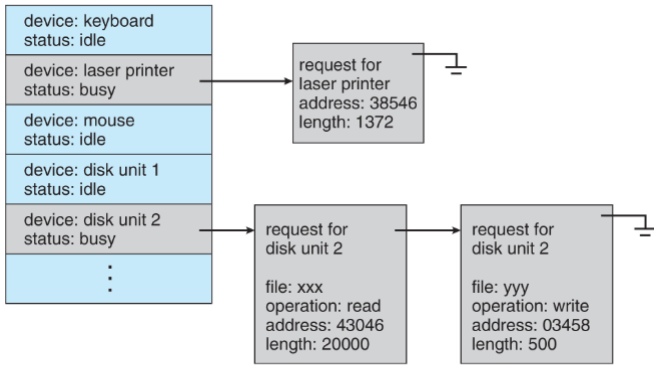
\includegraphics[width=\linewidth]{./content/OS_Internals/images/2026-03-31-17-37-10.png}
%   \end{minipage}%
%   \hfill
%   \begin{minipage}[t]{0.45\linewidth}
%     \section{Common PC and Data-center I/O devices and Interface Speeds}
%     \centering
%     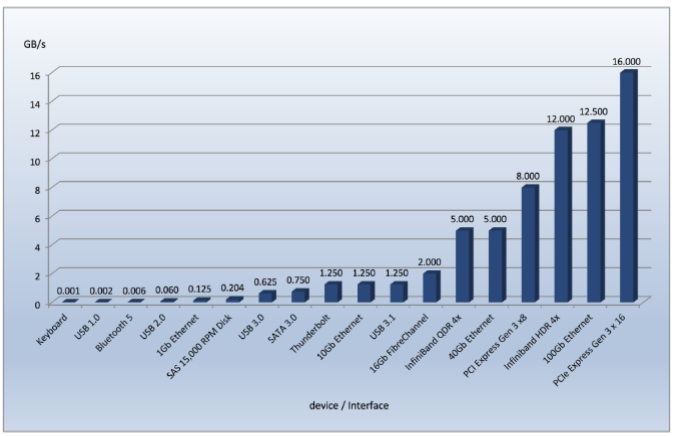
\includegraphics[width=0.5\linewidth]{./content/OS_Internals/images/2026-03-31-17-37-28.png}
%   \end{minipage}
% \end{center}

% \section{Kernel I/O Subsystem (Cont.)}

% \subsubsection{Caching} - faster device holding copy of data
% \begin{itemize}
%   \item Always just a copy
%   \item Key to performance
%   \item Sometimes combined with buffering
% \end{itemize}

% \subsubsection{Spooling} - hold output for a device
% \begin{itemize}
%   \item If device can serve only one request at a time
%   \item i.e., Printing
% \end{itemize}

% \subsubsection{Device reservation} - provides exclusive access to a device
% \begin{itemize}
%   \item System calls for allocation and de-allocation
%   \item Watch out for deadlock
% \end{itemize}

% \section{Error Handling}

% OS can recover from disk read, device unavailable, transient write failures
% \begin{itemize}
%   \item Retry a read or write, for example
%   \item Some systems more advanced - Solaris FMA, AIX.  Track error frequencies, stop using device with increasing frequency of retry-able errors
% \end{itemize}

% Most return an error number or code when I/O request fails
% System error logs hold problem reports

% \section{I/O Protection}

% User process may accidentally or purposefully attempt to disrupt normal operation via illegal I/O instructions
% \begin{itemize}
%   \item All I/O instructions defined to be privileged
%   \item I/O must be performed via system calls. Memory-mapped and I/O port memory locations must be protected too
% \end{itemize}

% \section{Use of a System Call to Perform I/O}

% \begin{figure}[h!]
%   \centering
%   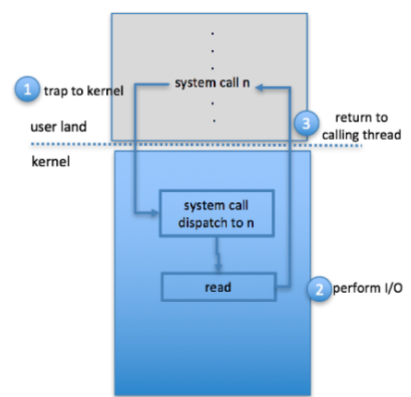
\includegraphics[width=0.35\linewidth]{./content/OS_Internals/images/2026-03-31-17-38-05.png}
% \end{figure}


% \section{Kernel Data Structures}

% Kernel keeps state info for I/O components, including open file tables, network connections, character device state

% Many, many complex data structures to track buffers, memory allocation, "dirty" blocks

% Some use object-oriented methods and message passing to implement I/O.


% Windows uses message passing:
% \begin{itemize}
%   \item Message with I/O information passed from user mode into kernel
%   \item Message modified as it flows through to device driver and back to process
%   \item Pros/cons?
% \end{itemize}

% \section{UNIX I/O Kernel Structure}

% \begin{figure}[h!]
%   \centering
%   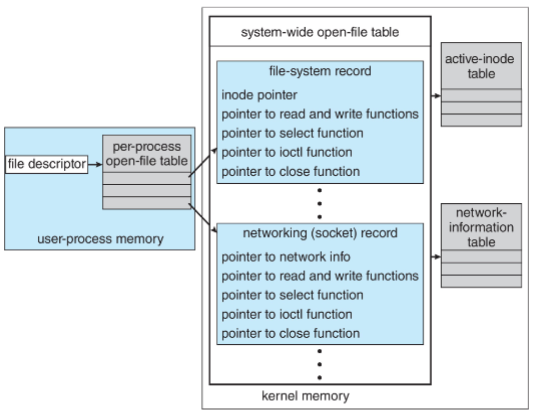
\includegraphics[width=0.35\linewidth]{./content/OS_Internals/images/2026-03-31-17-38-25.png}
% \end{figure}

% \section{Power Management}

% Not strictly domain of I/O, but much is I/O related
% Computers and devices use electricity, generate heat, frequently require cooling
% OSes can help manage and improve use

% Cloud computing environments move virtual machines between servers. Can end up evacuating whole systems and shutting them down

% Mobile computing has power management as first class OS aspect


% For example, Android implements component:

% \begin{itemize}
%   \item level power management:
%         \begin{itemize}
%           \item[] Understands relationship between components
%           \item[] Build device tree representing physical device topology
%           \item[] System bus -> I/O subsystem -> \{flash, USB storage\}
%           \item[] Device driver tracks state of device, whether in use
%           \item[] Unused component - turn it off
%           \item[] All devices in tree branch unused - turn off branch
%         \end{itemize}
%   \item Wake locks - like other locks but prevent sleep of device when lock is held
%   \item Power collapse - put a device into very deep sleep
%         \begin{itemize}
%           \item[] Marginal power use
%           \item[] Only awake enough to respond to external stimuli (button press, incoming call)
%         \end{itemize}
% \end{itemize}


% Modern systems use advanced configuration and power interface (ACPI) firmware providing code that runs as routines called by kernel for device discovery, management, error and power management

% \section{Kernel I/O Subsystem Summary}

% In summary, the I/O subsystem coordinates an extensive collection of services that are available to applications and to other parts of the kernel
% \begin{itemize}
%   \item Management of the name space for files and devices
%   \item Access control to files and devices
%   \item Operation control (for example, a modem cannot seek())
%   \item File-system space allocation
%   \item Device allocation
%   \item Buffering, caching, and spooling
%   \item I/O scheduling
%   \item Device-status monitoring, error handling, and failure recovery
%   \item Device-driver configuration and initialization
%   \item Power management of I/O devices
% \end{itemize}

% The upper levels of the I/O subsystem access devices via the uniform interface provided by the device drivers

% \section{Transforming I/O Requests to Hardware Operations}

% Consider reading a file from disk for a process
% \begin{itemize}
%   \item Determine device holding file
%   \item Translate name to device representation
%   \item Physically read data from disk into buffer
%   \item Make data available to requesting process
%   \item Return control to process
% \end{itemize}

% \section{Life Cycle of An I/O Request}

% \begin{figure}[h!]
%   \centering
%   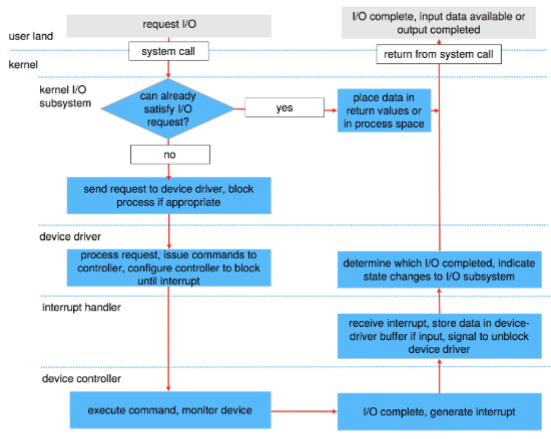
\includegraphics[width=0.5\linewidth]{./content/OS_Internals/images/2026-03-31-17-38-53.png}
% \end{figure}


% \section{STREAMS}


% \begin{flushleft}
%   \begin{minipage}{0.65\linewidth}
%     \raggedright
%     STREAM - a full-duplex communication channel between a user-level process and a device in Unix System V and beyond

%     A STREAM consists of
%     \begin{itemize}
%       \item STREAM head interfaces with the user process
%       \item driver end interfaces with the device
%       \item zero or more STREAM modules between them
%     \end{itemize}

%     Each module contains a read queue and a write queue
%     Message passing is used to communicate between queues
%     Flow control option to indicate available or busy
%     Asynchronous internally, synchronous where user process communicates with stream head

%   \end{minipage}%
%   \hfill
%   \begin{minipage}{0.3\linewidth}
%     \centering
%     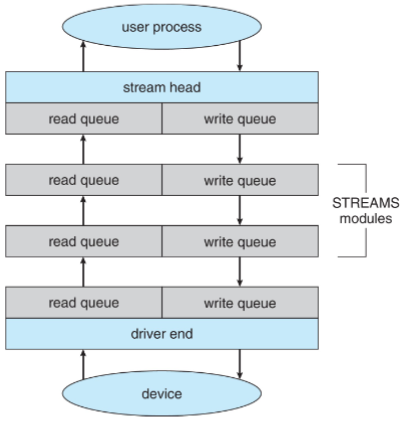
\includegraphics[width=\linewidth]{./content/OS_Internals/images/2026-03-31-17-39-39.png}
%     \captionof{figure}{The STREAMS Structure}
%   \end{minipage}
% \end{flushleft}


% \section{Performance}

% I/O a major factor in system performance
% \begin{itemize}
%   \item Demands CPU to execute device driver, kernel I/O code
%   \item Context switches due to interrupts
%   \item Data copying
%   \item Network traffic especially stressful
% \end{itemize}

% \section{Intercomputer Communications}

% \begin{figure}[h!]
%   \centering
%   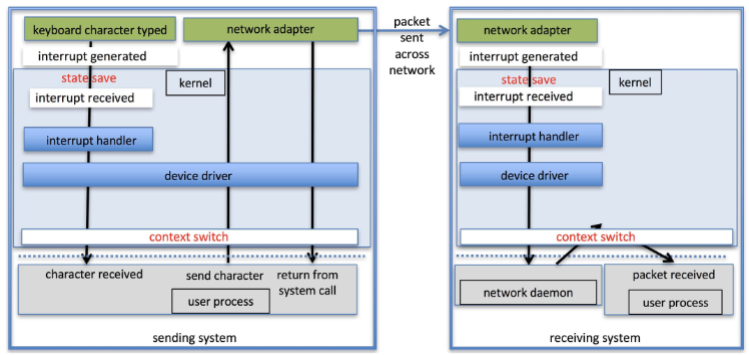
\includegraphics[width=0.5\linewidth]{./content/OS_Internals/images/2026-03-31-17-40-43.png}
% \end{figure}


% \section{Improving Performance}

% \begin{itemize}
%   \item Reduce number of context switches
%   \item Reduce data copying
%   \item Reduce interrupts by using large transfers, smart controllers, polling  650]
%   \item Use DMA
%   \item Use smarter hardware devices
%   \item Balance CPU, memory, bus, and I/O performance for highest throughput
%   \item Move user-mode processes / daemons to kernel threads
% \end{itemize}

% \begin{center}
%   \begin{minipage}[t]{0.45\linewidth}
%     \section{Device-Functionality Progression}
%     \centering
%     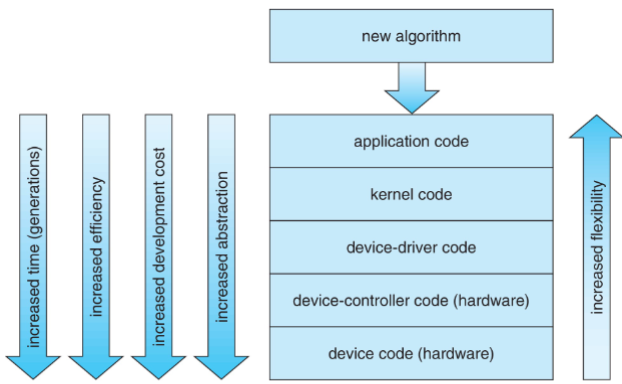
\includegraphics[width=\linewidth]{./content/OS_Internals/images/2026-03-31-17-41-05.png}
%   \end{minipage}%
%   \hfill
%   \begin{minipage}[t]{0.45\linewidth}
%     \section{I/O Performance of Storage (and Network Latency)}
%     \centering
%     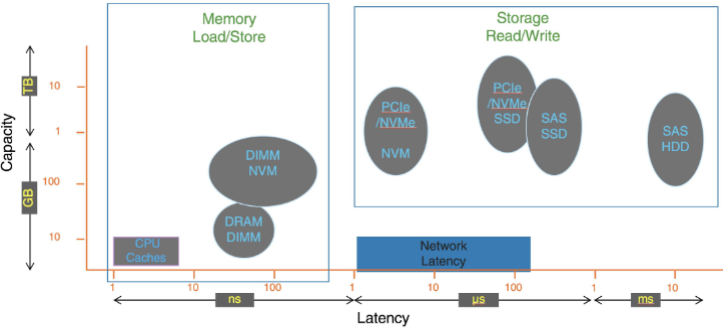
\includegraphics[width=0.5\linewidth]{./content/OS_Internals/images/2026-03-31-17-41-46.png}
%   \end{minipage}
% \end{center}
\section{Panoramica}
(fatto alla velox, ma alcune domande all'esame ci possono essere)
La gestione dell'I/O è un componente principale della progettazione e del funzionamento dei sistemi operativi.

\begin{itemize}
  \item Aspetto importante del funzionamento del computer
  \item I dispositivi di I/O variano notevolmente
  \item Vari metodi per controllarli
  \item Gestione delle prestazioni (Performance management)
  \item Frequente introduzione di nuovi tipi di dispositivi
\end{itemize}

Porte, bus e device controller si connettono a vari dispositivi.
I device driver incapsulano i dettagli del dispositivo, presentando un'interfaccia di accesso uniforme al sottosistema di I/O.

\section{I/O Hardware}

Incredibile varietà di dispositivi di I/O come: storage, trasmissione, interfacce umane.

Concetti comuni - i segnali dai dispositivi di I/O si interfacciano con il computer:

\begin{flushleft}
  \begin{minipage}{0.65\linewidth}
    \raggedright
    \begin{itemize}
      \item \textbf{Porta (Port):} - punto di connessione per il dispositivo
      \item \textbf{Bus:} - daisy chain o accesso diretto condiviso
            \begin{itemize}
              \item[-] \textbf{PCI:} - bus comune nei PC e nei server, PCI Express (PCIe)
              \item[-] \textbf{expansion bus} - connette dispositivi relativamente lenti
              \item[-] \textbf{Serial-attached SCSI (SAS)} - interfaccia comune per dischi
            \end{itemize}
      \item \textbf{Controller (host adapter)} - elettronica che gestisce porta, bus, dispositivo:
            \begin{itemize}
              \item[-] A volte integrato
              \item[-] A volte su una scheda a circuito separata (host adapter)
              \item[-] Contiene processore, microcodice, memoria privata, bus controller, ecc.
                    Alcuni comunicano con il controller specifico del dispositivo tramite bus controller, microcodice, memoria,
                    ecc.
            \end{itemize}
    \end{itemize}
  \end{minipage}%
  \hfill
  \begin{minipage}{0.3\linewidth}
    \centering
    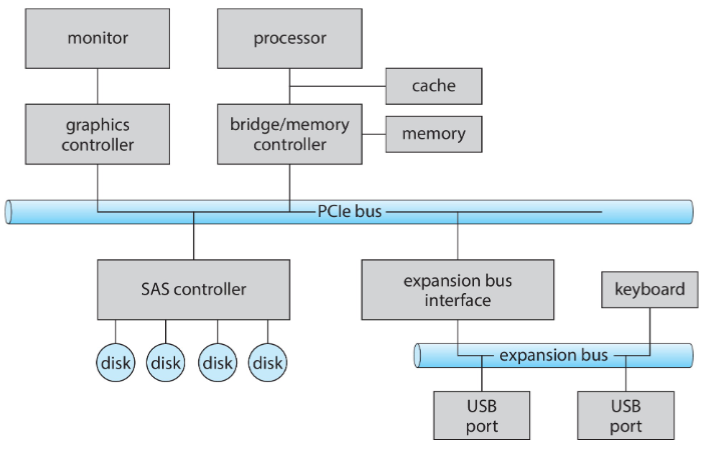
\includegraphics[width=\linewidth]{content/OS_Internals/images/2026-03-31-16-53-40.png}
  \end{minipage}
\end{flushleft}


\begin{flushleft}
  \begin{minipage}{0.65\linewidth}
    \raggedright

    Il Fibre channel (FC) è un controller complesso, solitamente una scheda a
    circuito separata (host-bus adapter, HBA) collegata al bus.

    Le istruzioni di I/O controllano i dispositivi.

    I dispositivi solitamente hanno registri in cui il device driver inserisce
    comandi, indirizzi e dati da scrivere, o legge dati dai
    registri dopo l'esecuzione del comando.

    \begin{itemize}
      \item Registro data-in, registro data-out, registro di stato (status register), registro di controllo (control register)
      \item Tipicamente 1-4 byte, o buffer FIFO
    \end{itemize}

    I dispositivi hanno indirizzi, utilizzati da: Istruzioni di I/O dirette o
    Memory-mapped I/O (MMIO - il dispositivo si prende un pezzo di memoria, non c'è ram
    ma c'è il dispositivi diverso da quello che verrà presentato nei prossimi capitoli),
    dati del dispositivo e registri di comando mappati nello
    spazio degli indirizzi del processore, specialmente per ampi spazi di indirizzamento (grafica).


  \end{minipage}%
  \hfill
  \begin{minipage}{0.3\linewidth}
    \centering
    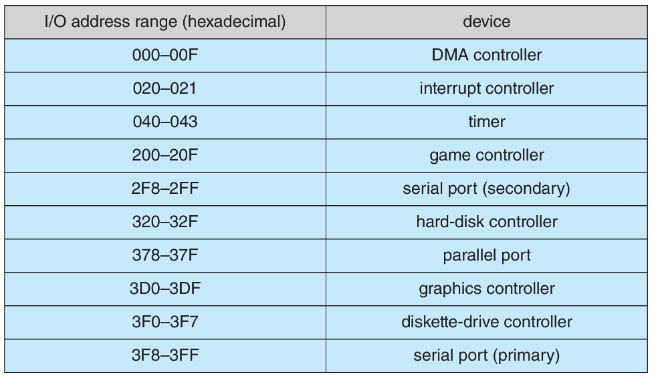
\includegraphics[width=\linewidth]{content/OS_Internals/images/2026-03-31-16-57-08.png}
    \captionof{figure}{Posizioni delle porte di I/O dei dispositivi sui PC (parziale)}
  \end{minipage}
\end{flushleft}

\section{Polling}
(Parte interessante)

In memoria secondaria bisogna controllare se il disco è pronto, se è occupato, etc.

Per ogni byte di I/O:

\begin{enumerate}
  \item Legge il bit di busy dal registro di stato finché non è 0
  \item L'host imposta il bit di lettura o scrittura e, se in scrittura, copia i dati nel registro data-out
  \item L'host imposta il bit command-ready
  \item Il controller imposta il bit di busy, esegue il trasferimento
  \item Il controller azzera il bit di busy, il bit di errore, il bit command-ready al termine del trasferimento
\end{enumerate}

Il passo 1 è un ciclo di busy-wait per attendere l'I/O dal dispositivo. Questo è ragionevole se il dispositivo è veloce, ma inefficiente se il dispositivo è lento.

La CPU passa ad altri task? Ma se salta un ciclo, i dati vengono sovrascritti / persi.

\section{Interrupt}
Il polling può avvenire in 3 cicli di istruzione.
Leggi lo stato, AND logico per estrarre il bit di stato, salta se non è zero. Come essere
più efficienti se è diverso da zero solo raramente?


Linea Interrupt-request della CPU attivata dal dispositivo di I/O, controllata dal processore dopo ogni istruzione.

\begin{itemize}
  \item L'\textbf{Interrupt handler} riceve gli interrupt; possono essere \textbf{mascherabili} (maskable) per ignorare o ritardare alcuni interrupt
  \item \textbf{Interrupt vector} per inviare l'interrupt all'handler corretto. Context switch all'inizio e alla fine basato sulla priorità, alcuni non mascherabili.
        Interrupt chaining se c'è più di un dispositivo con lo stesso numero di interrupt
\end{itemize}


\begin{flushleft}
  \begin{minipage}{0.7\linewidth}
    \raggedright

    Meccanismo di interrupt utilizzato anche per le eccezioni: terminare un processo, crash del sistema a causa di un errore hardware.


    Il page fault viene eseguito in caso di errore di accesso alla memoria.
    Le system call vengono eseguite tramite trap per attivare il kernel all'esecuzione della
    richiesta.

    I sistemi Multi-CPU possono elaborare gli interrupt in modo concorrente, se il sistema operativo è progettato per gestirlo.

    Utilizzato per elaborazioni sensibili al tempo, frequenti, deve essere veloce.


    Colori diversi sono attori diversi.

  \end{minipage}%
  \hfill
  \begin{minipage}{0.25\linewidth}
    \centering
    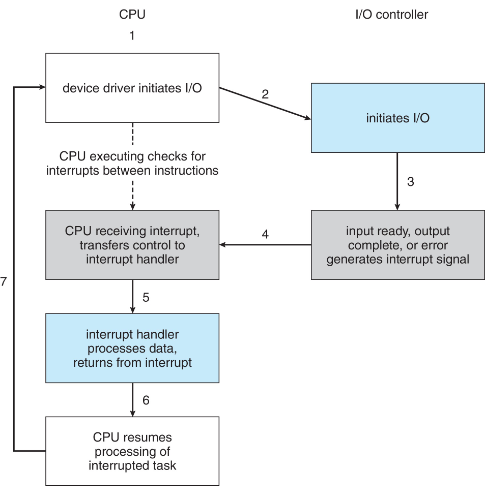
\includegraphics[width=\linewidth]{content/OS_Internals/images/2026-03-31-17-03-06.png}
  \end{minipage}
\end{flushleft}


\section{Latenza (Latency)}

Sottolineiamo la gestione degli interrupt perché anche i sistemi mono-utente
gestiscono centinaia di interrupt al secondo e i server centinaia di
migliaia.

Per esempio, un desktop macOS a riposo ha generato 23.000 interrupt in 10 secondi.

\section{Direct Memory Access (DMA)}






\begin{flushleft}
  \begin{minipage}{0.65\linewidth}
    \raggedright

    Utilizzato per evitare l'I/O programmato (un byte alla volta) per grandi spostamenti
    di dati. Richiede un controller DMA.

    Bypassa la CPU per trasferire i dati direttamente tra il dispositivo di I/O e la
    memoria. Tipo thread parallelo.


    Il sistema operativo scrive il blocco di comando DMA in memoria:

    \begin{itemize}
      \item Indirizzi di origine e destinazione
      \item Modalità di lettura o scrittura
      \item Conteggio dei byte
      \item Scrive la posizione del blocco di comandi nel controller DMA
      \item Bus mastering del controller DMA - prende il controllo del bus dalla CPU. Ruba cicli (Cycle stealing) alla CPU ma è comunque molto più efficiente
      \item Al termine, lancia un interrupt per segnalare il completamento
    \end{itemize}

    Una versione consapevole degli indirizzi virtuali può essere ancora più efficiente -
    DVMA.
  \end{minipage}%
  \hfill
  \begin{minipage}{0.3\linewidth}
    \centering
    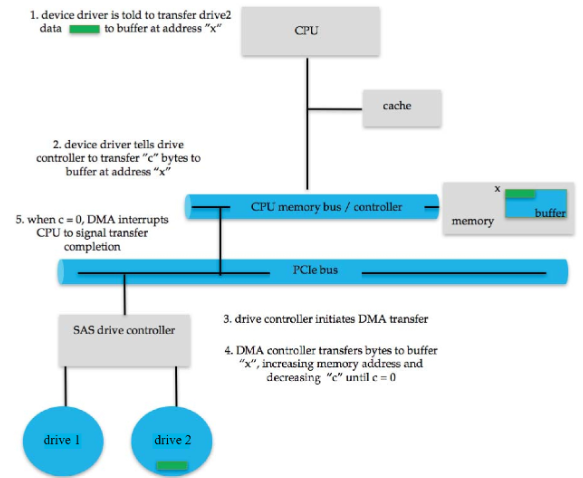
\includegraphics[width=\linewidth]{content/OS_Internals/images/2026-03-31-17-09-14.png}
    \captionof{figure}{Processo in sei fasi per eseguire un trasferimento DMA}
  \end{minipage}
\end{flushleft}



\section{Interfaccia di I/O per le applicazioni}

Le system call di I/O incapsulano i comportamenti dei dispositivi in classi generiche.
Il livello dei device-driver nasconde le differenze tra i controller di I/O al kernel.
Nuovi dispositivi che comunicano con protocolli già implementati non richiedono lavoro aggiuntivo.
Ogni sistema operativo ha le proprie strutture del sottosistema di I/O e framework per i device driver.
I dispositivi variano in molte dimensioni:

\begin{flushleft}
  \begin{minipage}{0.65\linewidth}
    \raggedright
    \begin{itemize}
      \item Stream di caratteri o a blocchi (Character-stream o block)
      \item Sequenziale o ad accesso casuale (random-access)
      \item Sincrono o asincrono (o entrambi)
      \item Condivisibile (Sharable) o dedicato
      \item Velocità operativa
      \item lettura-scrittura, sola lettura, o sola scrittura
    \end{itemize}
  \end{minipage}%
  \hfill
  \begin{minipage}{0.3\linewidth}
    \centering
    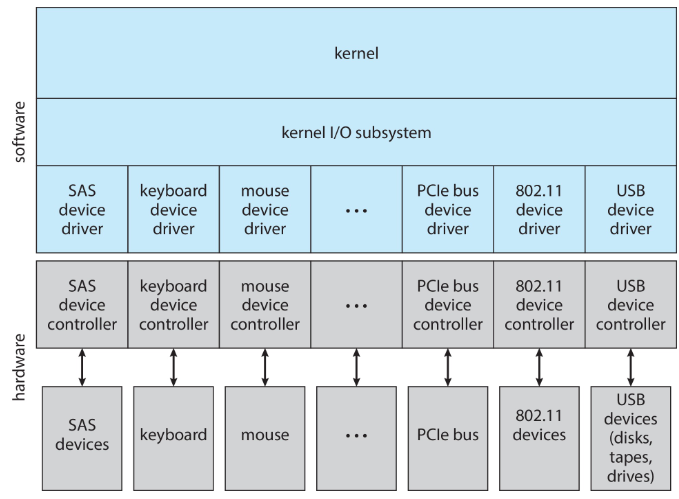
\includegraphics[width=\linewidth]{content/OS_Internals/images/2026-03-31-17-11-50.png}
  \end{minipage}
\end{flushleft}


\section{Caratteristiche dei dispositivi di I/O}

\begin{table}[h!]
  \renewcommand{\arraystretch}{1.5}
  \centering
  \begin{tabular}{p{3.5cm} p{5.5cm} p{4.5cm}}
    \hline
    \textbf{Aspetto}                 & \textbf{Variazione}                                                                                  & \textbf{Esempio}                                  \\
    \hline
    modalità di trasferimento dati   & carattere \newline blocco                                                                            & terminale \newline disco                          \\
    metodo di accesso                & sequenziale \newline casuale                                                                         & modem \newline CD-ROM                             \\
    pianificazione del trasferimento & sincrono \newline asincrono                                                                          & nastro \newline tastiera                          \\
    condivisione                     & dedicato \newline condivisibile                                                                      & nastro \newline tastiera                          \\
    velocità del dispositivo         & latenza \newline tempo di seek \newline velocità di trasferimento \newline ritardo tra le operazioni &                                                   \\
    direzione di I/O                 & sola lettura \newline sola scrittura \newline lettura-scrittura                                      & CD-ROM \newline controller grafico \newline disco \\
    \hline
  \end{tabular}
\end{table}


\begin{figure}[h!]
  \centering
  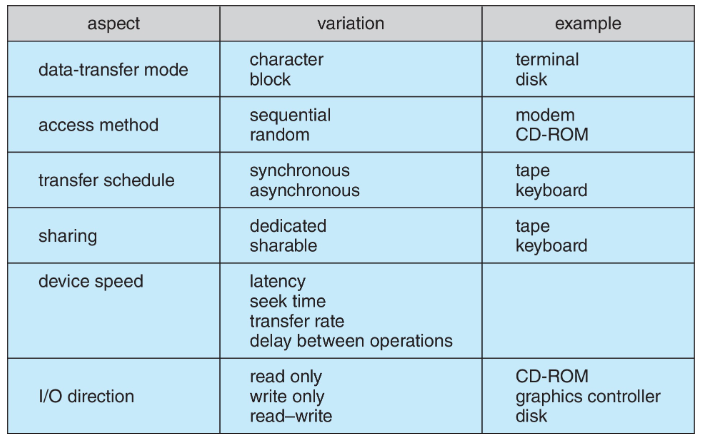
\includegraphics[width=0.25\linewidth]{content/OS_Internals/images/2026-03-31-17-12-50.png}
\end{figure}


Le sottigliezze dei dispositivi sono gestite dai device driver.
In generale i dispositivi di I/O possono essere raggruppati dal sistema operativo in

\begin{itemize}
  \item Block I/O (I/O a blocchi)
  \item Character I/O (I/O a caratteri / Stream)
  \item Accesso a file mappati in memoria (Memory-mapped file access)
  \item Socket di rete
\end{itemize}

Per la manipolazione diretta delle caratteristiche specifiche del dispositivo di I/O, di solito c'è una scappatoia / porta di servizio (back door).
Chiamata Unix ioctl() per inviare bit arbitrari a un registro di controllo del dispositivo e dati al registro dati del dispositivo.
UNIX e Linux usano tuple di numeri di dispositivo "major" e "minor" per identificare il tipo e l'istanza dei dispositivi (qui major 8 e minor 0-4):

\begin{verbatim}
% ls -l /dev/sda* brw-rw---- 1 root disk 8, 0 Mar 16 09:18 /dev/sda 
brw-rw---- 1 root disk 8, 1 Mar 16 09:18 /dev/sda1 
brw-rw---- 1 root disk 8, 2 Mar 16 09:18 /dev/sda2 
brw-rw---- 1 root disk 8, 3 Mar 16 09:18 /dev/sda3 
\end{verbatim}

\section{Dispositivi a blocchi e a caratteri}

I dispositivi a blocchi includono le unità disco (disk drives)
\begin{itemize}
  \item I comandi includono read, write, seek
  \item Raw I/O, I/O diretto, o accesso al file system
  \item Accesso tramite memory-mapped file possibile: File mappato nella memoria virtuale e cluster portati tramite demand paging
  \item DMA
\end{itemize}

I dispositivi a caratteri includono tastiere, mouse, porte seriali
\begin{itemize}
  \item I comandi includono get(), put()
  \item Librerie stratificate al di sopra permettono l'editing di linea
\end{itemize}

\section{Dispositivi di rete}

Variano abbastanza da quelli a blocchi e a caratteri da avere una propria interfaccia.
Linux, Unix, Windows e molti altri includono l'interfaccia socket

\begin{itemize}
  \item Separa il protocollo di rete dall'operazione di rete
  \item Include la funzionalità select()
\end{itemize}
Gli approcci variano ampiamente (pipe, FIFO, stream, code, mailbox)

\section{Clock e Timer}

Forniscono ora corrente, tempo trascorso, timer.
Risoluzione normale circa 1/60 di secondo. Alcuni sistemi forniscono timer
a risoluzione più alta. Timer a intervallo programmabile utilizzato per tempistiche, interrupt periodici.

\verb|ioctl()| (su UNIX) copre aspetti particolari dell'I/O come clock e timer

\section{I/O Non bloccante e Asincrono}

\subsubsection{Bloccante (Blocking) - processo sospeso fino al completamento dell'I/O}
\begin{itemize}
  \item Facile da usare e comprendere
  \item Insufficiente per alcune necessità
\end{itemize}

\subsubsection{Non bloccante (Nonblocking) - la chiamata di I/O restituisce tutto ciò che è disponibile}
\begin{itemize}
  \item Interfaccia utente, copia di dati (I/O bufferizzato)
  \item Implementato tramite multi-threading
  \item Ritorna rapidamente con il conteggio dei byte letti o scritti
  \item select() per verificare se i dati sono pronti, quindi read() o write() per il trasferimento
\end{itemize}

\subsubsection{Asincrono (Asynchronous) - il processo continua l'esecuzione mentre l'I/O viene eseguito}
\begin{itemize}
  \item Difficile da usare
  \item Il sottosistema di I/O segnala al processo quando l'I/O è completato
\end{itemize}

\section{Due metodi di I/O}

\begin{figure}[h!]
  \centering
  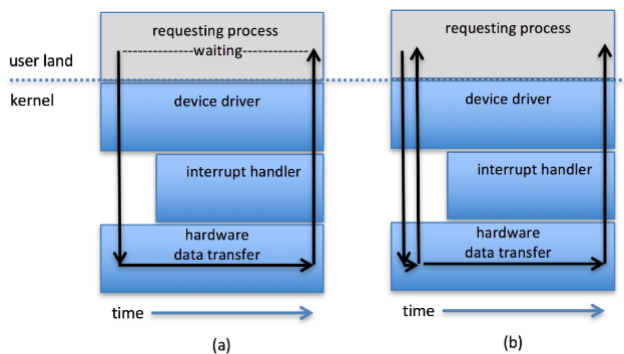
\includegraphics[width=0.25\linewidth]{./content/OS_Internals/images/2026-03-31-17-36-35.png}
\end{figure}

\section{Vectored I/O}
(saltato)

Il Vectored I/O consente a una singola system call di eseguire più operazioni di I/O.

Ad esempio, Unix readve() accetta un vettore di buffer multipli in cui leggere o da cui scrivere.

Questo metodo scatter-gather è migliore di molteplici chiamate I/O individuali
\begin{itemize}
  \item Riduce il context switching e l'overhead delle system call
  \item Alcune versioni forniscono atomicità. Evita, per esempio, di preoccuparsi di thread multipli che modificano i dati mentre si verificano letture/scritture
\end{itemize}

\section{Sottosistema di I/O del Kernel}

\begin{flushleft}
  \begin{minipage}[t]{0.48\linewidth}
    \raggedright
    \subsubsection{Scheduling}
    \begin{itemize}
      \item Un certo ordinamento delle richieste di I/O tramite coda per-dispositivo
      \item Alcuni SO tentano di garantire l'equità (fairness)
      \item Alcuni implementano la Quality Of Service (es. IPQOS)
    \end{itemize}
  \end{minipage}%
  \hfill
  \begin{minipage}[t]{0.48\linewidth}
    \raggedright
    \subsubsection{Buffering: memorizzare i dati in memoria durante il trasferimento tra dispositivi}
    \begin{itemize}
      \item Per far fronte alla mancata corrispondenza della velocità del dispositivo
      \item Per far fronte alla mancata corrispondenza della dimensione di trasferimento del dispositivo
      \item Per mantenere la "semantica di copia" (copy semantics)
      \item Double buffering - due copie dei dati: Kernel e utente, Dimensioni variabili, Pieno / in elaborazione e non-pieno / in uso, Il Copy-on-write può essere usato per l'efficienza in alcuni casi
    \end{itemize}
  \end{minipage}
\end{flushleft}


\begin{center}
  \begin{minipage}{1\linewidth}
    \begin{minipage}[t]{0.47\linewidth}
      \section{Device-status Table}
      \centering
      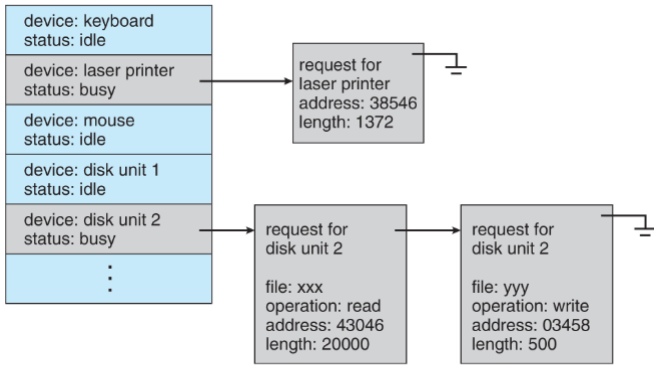
\includegraphics[width=0.6\linewidth]{./content/OS_Internals/images/2026-03-31-17-37-10.png}
    \end{minipage}%
    \hfill
    \begin{minipage}[t]{0.47\linewidth}
      \section{Velocità disp. I/O}
      \centering
      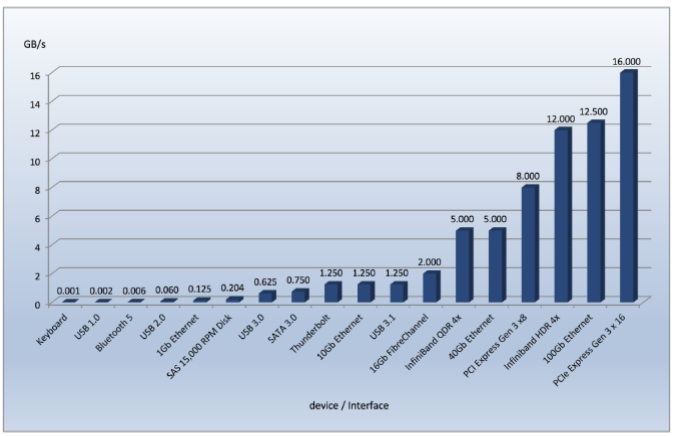
\includegraphics[width=0.4\linewidth]{./content/OS_Internals/images/2026-03-31-17-37-28.png}
    \end{minipage}
  \end{minipage}
\end{center}

nota: gli osbook  tutti e os161 intor memory overview sincro

file, user process e IO fanno riferimento ai lab ma non li chiede

gli es su os161 comprendono anche lab5 ma non è programma (no file system).


OS161 -> esercizio da esami hai fatto il lab? come si risolve il problema?

% \section{Sottosistema di I/O del Kernel (Cont.)}

% ! NON  l'ha fatto

% \paragraph{Caching} - dispositivo più veloce che mantiene una copia dei dati
% \begin{itemize}
%   \item Sempre solo una copia
%   \item Fondamentale per le prestazioni
%   \item A volte combinato con il buffering
% \end{itemize}

% \paragraph{Spooling} - trattiene l'output per un dispositivo
% \begin{itemize}
%   \item Se il dispositivo può servire solo una richiesta alla volta
%   \item es. Stampa
% \end{itemize}

% \paragraph{Prenotazione del dispositivo (Device reservation)} - fornisce accesso esclusivo a un dispositivo
% \begin{itemize}
%   \item System call per l'allocazione e la de-allocazione
%   \item Attenzione ai deadlock
% \end{itemize}

% \section{Gestione degli errori (Error Handling)}

% Il SO può riprendersi da errori di lettura del disco, dispositivo non disponibile, fallimenti di scrittura transitori
% \begin{itemize}
%   \item Riprovare una lettura o una scrittura, per esempio
%   \item Alcuni sistemi sono più avanzati - Solaris FMA, AIX. Tracciano le frequenze degli errori, smettono di usare il dispositivo se aumenta la frequenza di errori riprovabili (retry-able errors)
% \end{itemize}

% La maggior parte restituisce un numero o codice di errore quando una richiesta di I/O fallisce.
% I log di sistema degli errori conservano i report dei problemi.

% \section{Protezione dell'I/O}

% Un processo utente potrebbe tentare accidentalmente o intenzionalmente di interrompere le normali operazioni tramite istruzioni di I/O illegali
% \begin{itemize}
%   \item Tutte le istruzioni di I/O sono definite come privilegiate
%   \item L'I/O deve essere eseguito tramite system call. Anche le locazioni di memoria mappate in memoria e le porte di I/O devono essere protette
% \end{itemize}

% \section{Uso di una System Call per eseguire l'I/O}

% \begin{figure}[h!]
%   \centering
%   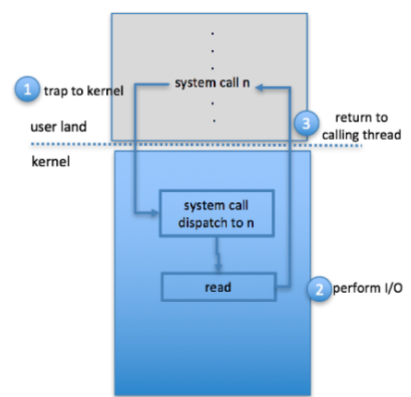
\includegraphics[width=0.25\linewidth]{./content/OS_Internals/images/2026-03-31-17-38-05.png}
% \end{figure}


% \section{Strutture Dati del Kernel}

% Il Kernel mantiene informazioni di stato per i componenti di I/O, comprese tabelle dei file aperti, connessioni di rete, stato dei dispositivi a caratteri.

% Molteplici strutture dati complesse per tracciare buffer, allocazione di memoria, blocchi "sporchi" (dirty blocks).

% Alcuni usano metodi orientati agli oggetti e passaggio di messaggi (message passing) per implementare l'I/O.


% Windows usa il message passing:
% \begin{itemize}
%   \item Il messaggio con le informazioni di I/O passa dalla modalità utente al kernel
%   \item Il messaggio viene modificato mentre scorre fino al device driver e torna al processo
%   \item Pro/contro?
% \end{itemize}


% \newpage
% \section{Struttura del Kernel di I/O in UNIX}

% \begin{figure}[h!]
%   \centering
%   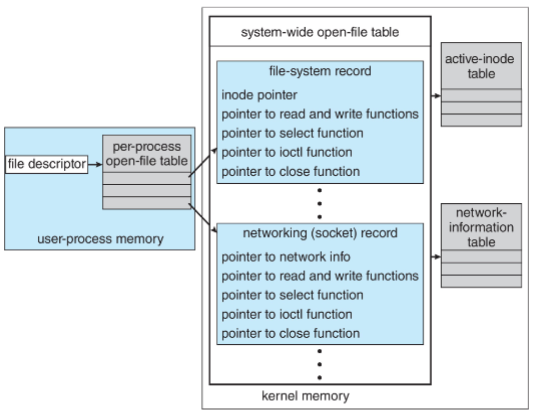
\includegraphics[width=0.35\linewidth]{./content/OS_Internals/images/2026-03-31-17-38-25.png}
% \end{figure}

% \section{Gestione dell'energia (Power Management)}

% Non è strettamente dominio dell'I/O, ma gran parte è correlato all'I/O.
% I computer e i dispositivi usano elettricità, generano calore, spesso richiedono raffreddamento.
% I sistemi operativi possono aiutare a gestirne e migliorarne l'uso.

% Gli ambienti di Cloud computing spostano macchine virtuali tra i server. Possono finire per evacuare interi sistemi e spegnerli.

% Il mobile computing ha il power management come aspetto di primaria importanza nel SO.


% Per esempio, Android implementa a livello di componente:

% \begin{itemize}
%   \item level power management (gestione dell'energia a livello di componente):
%         \begin{itemize}
%           \item[] Comprende la relazione tra i componenti
%           \item[] Costruisce l'albero dei dispositivi che rappresenta la topologia fisica dei dispositivi
%           \item[] System bus -> Sottosistema I/O -> \{flash, USB storage\}
%           \item[] Il device driver tiene traccia dello stato del dispositivo, se è in uso
%           \item[] Componente non utilizzato - lo spegne
%           \item[] Tutti i dispositivi in un ramo dell'albero non sono utilizzati - spegne il ramo
%         \end{itemize}
%   \item Wake locks - come altri lock, ma prevengono la sospensione (sleep) del dispositivo quando il lock è mantenuto
%   \item Power collapse - mette un dispositivo in un sonno molto profondo (very deep sleep)
%         \begin{itemize}
%           \item[] Uso di energia marginale
%           \item[] Sveglio solo quel tanto che basta per rispondere agli stimoli esterni (pressione di un pulsante, chiamata in arrivo)
%         \end{itemize}
% \end{itemize}


% I sistemi moderni utilizzano un firmware ACPI (Advanced Configuration and Power Interface) che fornisce codice che viene eseguito come routine chiamate dal kernel per il rilevamento del dispositivo, la gestione, gli errori e la gestione dell'alimentazione.

% \section{Riepilogo del Sottosistema di I/O del Kernel}

% In sintesi, il sottosistema I/O coordina una vasta gamma di servizi disponibili per le applicazioni e per altre parti del kernel
% \begin{itemize}
%   \item Gestione dello spazio dei nomi per file e dispositivi
%   \item Controllo degli accessi a file e dispositivi
%   \item Controllo delle operazioni (per esempio, un modem non può eseguire una seek())
%   \item Allocazione dello spazio nel file-system
%   \item Allocazione dei dispositivi
%   \item Buffering, caching e spooling
%   \item Scheduling dell'I/O
%   \item Monitoraggio dello stato dei dispositivi, gestione degli errori e ripristino dai guasti
%   \item Configurazione e inizializzazione dei device-driver
%   \item Gestione energetica (Power management) dei dispositivi di I/O
% \end{itemize}

% I livelli superiori del sottosistema di I/O accedono ai dispositivi tramite l'interfaccia uniforme fornita dai device driver.

% \section{Trasformazione delle richieste di I/O in operazioni hardware}

% Consideriamo la lettura di un file dal disco per un processo
% \begin{itemize}
%   \item Determinare il dispositivo che contiene il file
%   \item Tradurre il nome nella rappresentazione del dispositivo
%   \item Leggere fisicamente i dati dal disco nel buffer
%   \item Rendere i dati disponibili al processo richiedente
%   \item Restituire il controllo al processo
% \end{itemize}

% \section{Ciclo di vita di una richiesta di I/O}

% \begin{figure}[h!]
%   \centering
%   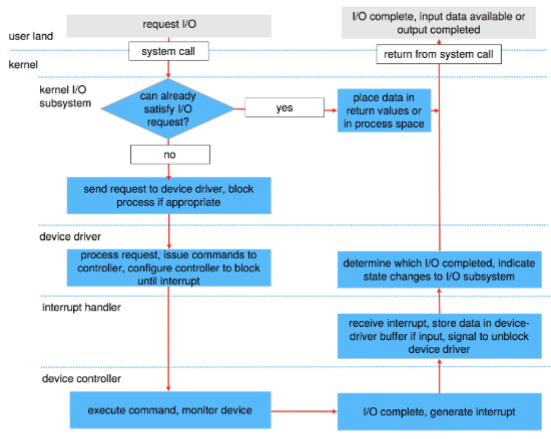
\includegraphics[width=0.25\linewidth]{./content/OS_Internals/images/2026-03-31-17-38-53.png}
% \end{figure}


% \section{STREAMS}


% \begin{flushleft}
%   \begin{minipage}{0.65\linewidth}
%     \raggedright
%     STREAM - un canale di comunicazione full-duplex tra un processo a livello utente e un dispositivo in Unix System V e successivi

%     Uno STREAM è composto da
%     \begin{itemize}
%       \item STREAM head che si interfaccia con il processo utente
%       \item driver end che si interfaccia con il dispositivo
%       \item zero o più moduli STREAM tra di loro
%     \end{itemize}

%     Ogni modulo contiene una coda di lettura e una coda di scrittura.
%     Il passaggio di messaggi (Message passing) viene utilizzato per comunicare tra le code.
%     Opzione di controllo di flusso (Flow control) per indicare disponibile o occupato.
%     Asincrono internamente, sincrono dove il processo utente comunica con lo stream head.

%   \end{minipage}%
%   \hfill
%   \begin{minipage}{0.3\linewidth}
%     \centering
%     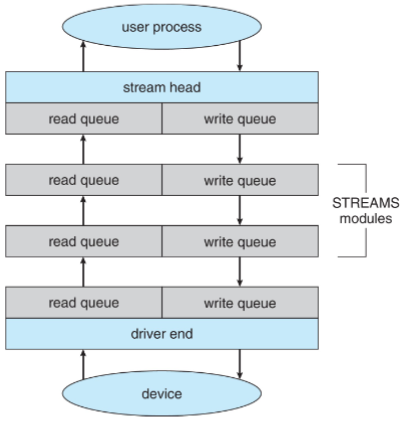
\includegraphics[width=\linewidth]{./content/OS_Internals/images/2026-03-31-17-39-39.png}
%     \captionof{figure}{La struttura degli STREAMS}
%   \end{minipage}
% \end{flushleft}


% \section{Prestazioni (Performance)}

% L'I/O è un fattore determinante per le prestazioni del sistema
% \begin{itemize}
%   \item Richiede la CPU per eseguire i device driver, il codice di I/O del kernel
%   \item Context switch causati dagli interrupt
%   \item Copia dei dati (Data copying)
%   \item Il traffico di rete è particolarmente gravoso
% \end{itemize}

% \section{Comunicazioni tra computer}

% \begin{figure}[h!]
%   \centering
%   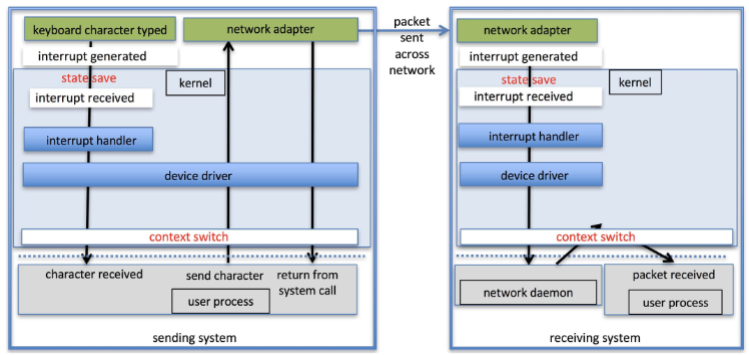
\includegraphics[width=0.5\linewidth]{./content/OS_Internals/images/2026-03-31-17-40-43.png}
% \end{figure}


% \section{Migliorare le prestazioni}

% \begin{itemize}
%   \item Ridurre il numero di context switch
%   \item Ridurre la copia dei dati
%   \item Ridurre gli interrupt utilizzando trasferimenti di grandi dimensioni, controller intelligenti, polling
%   \item Utilizzare il DMA
%   \item Utilizzare dispositivi hardware più intelligenti
%   \item Bilanciare le prestazioni di CPU, memoria, bus e I/O per ottenere il massimo throughput
%   \item Spostare processi in user-mode / demoni in kernel thread
% \end{itemize}

% \begin{center}
%   \begin{minipage}[t]{0.45\linewidth}
%     \section{Progressione delle funzionalità del dispositivo}
%     \centering
%     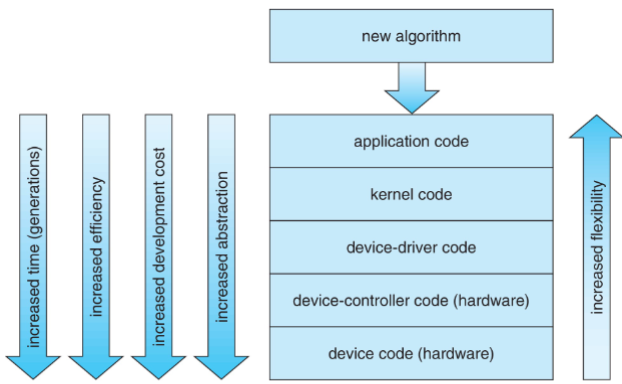
\includegraphics[width=0.8\linewidth]{./content/OS_Internals/images/2026-03-31-17-41-05.png}
%   \end{minipage}%
%   \hfill
%   \begin{minipage}[t]{0.45\linewidth}
%     \section{Prestazioni I/O dello Storage e Latenza Rete}
%     \centering
%     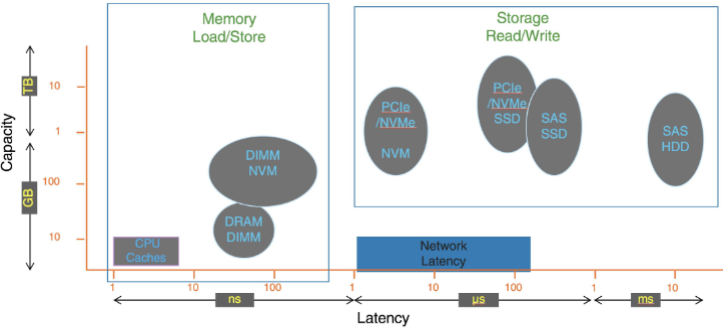
\includegraphics[width=0.8\linewidth]{./content/OS_Internals/images/2026-03-31-17-41-46.png}
%   \end{minipage}
% \end{center}